\documentclass[a4paper,oneside,12pt]{extreport}

\usepackage{mmap}
\usepackage[T2A]{fontenc}
\usepackage[utf8]{inputenc}
\usepackage[english,russian]{babel}

% Текст отчёта следует печатать, соблюдая следующие размеры полей:
% левое — 30 мм, правое — 15 мм, верхнее и нижнее — 20 мм.
\usepackage[left=20mm, right=15mm, top=15mm, bottom=15mm]{geometry}

% \setlength{\parindent}{1.25cm} % Абзацный отступ

\usepackage{setspace}
%\onehalfspacing % Полуторный интервал

\frenchspacing % Равномерные пробелы
\usepackage{indentfirst} % Красная строка

\usepackage{microtype}
\sloppy

\usepackage{titlesec}
\titlespacing*{\chapter}{0pt}{-30pt}{8pt}
\titlespacing*{\section}{\parindent}{*4}{*4}
\titlespacing*{\subsection}{\parindent}{*4}{*4}
\titleformat{\chapter}{\LARGE\bfseries}{\thechapter}{20pt}{\LARGE\bfseries}
\titleformat{\section}{\Large\bfseries}{\thesection}{40pt}{\Large\bfseries}

\usepackage{graphicx}
\usepackage{caption}

\usepackage[unicode,pdftex]{hyperref}
\hypersetup{hidelinks}

%% title begin
\usepackage{wrapfig}

\makeatletter
	\def\vhrulefill#1{\leavevmode\leaders\hrule\@height#1\hfill \kern\z@}
\makeatother
%% title end

%% begin code
\usepackage{listings}
\usepackage{xcolor}

\lstset{
	basicstyle=\footnotesize\ttfamily,
	breakatwhitespace=true,
	breaklines=true,
	commentstyle=\color{gray},
	frame=single,
	keywordstyle=\color{blue},
	showstringspaces=false,
	stringstyle=\color{red},
	tabsize=8
}

\lstdefinestyle{lispinline}{
	frame=none,
	language=Lisp
}

\newcommand{\code}[1]{\texttt{#1}}
%% end code

%% begin theorem
\usepackage{amsthm}

\makeatletter
\newtheoremstyle{indented}
	{}% measure of space to leave above the theorem
	{}% measure of space to leave below the theorem
	{}% name of font to use in the body of the theorem
	{\parindent}% measure of space to indent
	{\bfseries}% name of head font
	{.}% punctuation between head and body
	{ }% space after theorem head; " " = normal interword space
	{}% header specification (empty for default)
\makeatother

\theoremstyle{indented}

\newtheorem{definition}{Определение}[section]
\newtheorem{example}{Пример}[section]
\newtheorem{theorem}{Теорема}[section]
\newtheorem{task}{Задание}

\makeatletter
\DeclareRobustCommand\bfseriesitshape{%
	\not@math@alphabet\itshapebfseries\relax
	\fontseries\bfdefault
	\fontshape\itdefault
	\selectfont
}
\makeatother

\DeclareTextFontCommand{\textbfit}{\bfseriesitshape}
\DeclareTextFontCommand{\define}{\bfseriesitshape}
%% end theorem

%% begin columns
\usepackage{etoolbox,refcount}
\usepackage{multicol}

\newcounter{countitems}
\newcounter{nextitemizecount}
\newcommand{\setupcountitems}{%
	\stepcounter{nextitemizecount}%
	\setcounter{countitems}{0}%
	\preto\item{\stepcounter{countitems}}%
}
\makeatletter
\newcommand{\computecountitems}{%
	\edef\@currentlabel{\number\c@countitems}%
	\label{countitems@\number\numexpr\value{nextitemizecount}-1\relax}%
}
\newcommand{\nextitemizecount}{%
	\getrefnumber{countitems@\number\c@nextitemizecount}%
}
\newcommand{\previtemizecount}{%
	\getrefnumber{countitems@\number\numexpr\value{nextitemizecount}-1\relax}%
}
\makeatother
\newenvironment{AutoMultiColItemize}{%
	\ifnumcomp{\nextitemizecount}{>}{3}{\begin{multicols}{2}}{}%
		\setupcountitems\begin{itemize}}%
		{\end{itemize}%
		\unskip\computecountitems\ifnumcomp{\previtemizecount}{>}{3}{\end{multicols}}{}}
\makeatother
\newenvironment{AutoMultiColEnumerate}{%
	\ifnumcomp{\nextitemizecount}{>}{3}{\begin{multicols}{2}}{}%
		\setupcountitems\begin{enumerate}}%
		{\end{enumerate}%
		\unskip\computecountitems\ifnumcomp{\previtemizecount}{>}{3}{\end{multicols}}{}}
%% end columns

\usepackage{array}
\usepackage{float}
\restylefloat{table}

\usepackage{amsmath}
\usepackage{amssymb}

\begin{document}

\begin{titlepage}
	{\large % 14pt instead of 12pt
	\onehalfspacing
	\centering

	\begin{wrapfigure}[7]{l}{0.14\linewidth}
		\vspace{3mm}
		\hspace{-10mm}
		
\includegraphics[width=0.93\linewidth]{inc/img/bmstu-logo}
	\end{wrapfigure}
	{\singlespacing \footnotesize \bfseries Министерство науки и высшего образования Российской Федерации\\Федеральное государственное бюджетное образовательное учреждение\\высшего образования\\<<Московский государственный технический университет\\имени Н.~Э.~Баумана\\ (национальный исследовательский университет)>>\\(МГТУ им. Н.~Э.~Баумана)\\}

	\vspace{-2.2mm}
	\vhrulefill{0.9mm}\\
	\vspace{-7.5mm}
	\vhrulefill{0.2mm}\\
	\vspace{2mm}

	{\doublespacing \small \raggedright ФАКУЛЬТЕТ \hspace{25mm} «Информатика и системы управления»\\
	КАФЕДРА \hspace{5mm} «Программное обеспечение ЭВМ и информационные технологии»\\}

	\vspace{30mm}

	\textbf{ОТЧЁТ}\\
	По лабораторной работе №6\\
	По курсу: «Функциональное и логическое программирование»\\
	%Тема: «Тема работы»\\

	\vspace{60mm}

	\hspace{70mm} Студент:       \hfill Керимов~А.~Ш.\\
	\hspace{70mm} Группа:        \hfill ИУ7-64Б\\
	\hspace{70mm} Преподаватели: \hfill Толпинская~Н.~Б.,\\
	                             \hfill Строганов~Ю.~В.\\

	\vfill

	Москва\\
	\the\year\\}
\end{titlepage}

\setcounter{page}{2}


\section*{Практическая часть}

\begin{task}
	Дана функция \code{(defun mystery (x) (list (second x) (first x)))}.
	Какие результаты вычисления следующих выражений?
	\begin{AutoMultiColEnumerate}
		\item \begin{lstlisting}[style=lispinline, gobble=24]
			(mystery (one two))
			; (two one)
		\end{lstlisting}

		\item \begin{lstlisting}[style=lispinline, gobble=24]
			(mystery one 'two))
			; Invalid number of arguments: 2.
		\end{lstlisting}

		\item \begin{lstlisting}[style=lispinline, gobble=24]
			(mystery 'free)
			; The value FREE is not LIST.
		\end{lstlisting}

		\item \begin{lstlisting}[style=lispinline, gobble=24]
			(mystery (last 'one 'two))
			; The value ONE is not LIST.
		\end{lstlisting}
	\end{AutoMultiColEnumerate}
\end{task}

\begin{task}
	Написать функцию, которая переводит температуру в системе Фаренгейта температуру по Цельсию \code{(defun f-to-c (temp) ...)}.

	\begin{lstlisting}[language=Lisp, gobble=16]
		(defun f-to-c (temp)
		  (* (/ 5 9)
		     (- temp 32.0)))
	\end{lstlisting}
\end{task}

\begin{task}
	Что получится при вычисления каждого из выражений?
	\begin{AutoMultiColEnumerate}
		\item \begin{lstlisting}[style=lispinline, gobble=24]
			(list 'cons T Nil))
			; (cons T Nil)
		\end{lstlisting}

		\item \begin{lstlisting}[style=lispinline, gobble=24]
			(cons 'a (b c))
			; Undefined function: b.
		\end{lstlisting}

		\item \begin{lstlisting}[style=lispinline, gobble=24]
			(eval (eval (list 'cons T Nil)))
			; Undefined functionz: T
		\end{lstlisting}

		\item \begin{lstlisting}[style=lispinline, gobble=24]
			(apply #'cons '(T Nil))	
			; (T)
		\end{lstlisting}

		\item \begin{lstlisting}[style=lispinline, gobble=24]
			(list 'eval Nil)
			; (eval Nil)
		\end{lstlisting}

		\item \begin{lstlisting}[style=lispinline, gobble=24]
			(eval (list 'cons T Nil))
			; (T)
		\end{lstlisting}

		\item \begin{lstlisting}[style=lispinline, gobble=24]
			(eval Nil)
			; Nil
		\end{lstlisting}

		\item \begin{lstlisting}[style=lispinline, gobble=24]
			(eval (list 'eval NIL))
			; Nil
		\end{lstlisting}
	\end{AutoMultiColEnumerate}
\end{task}

\begin{task}
	Написать функцию, вычисляющую катет по заданной гипотенузе и другому катету прямоугольного треугольника, и составить диаграмму её вычисления.

	\begin{lstlisting}[language=Lisp, gobble=16]
		(defun cathetus (c b)
		  (sqrt
		    (- (* c c)
		       (* b b))))
	\end{lstlisting}
\end{task}

\begin{task}
	Написать функцию, вычисляющую площадь трапеции по ее основаниям и высоте, и составить диаграмму ее вычисления.
	\begin{lstlisting}[language=Lisp, gobble=16]
		(defun trapezoid-area (base1 base2 height)
		  (/
		    (*
		      (+ base1
		         base2)
		      height)
		    2.0))
	\end{lstlisting}
\end{task}

\section*{Теоретическая часть}

\subsection*{Как синтаксически представляется программа на Lisp}

В Lisp формы представления программы и обрабатываемых ею данных одинаковы (в виде S-выражений).
Поэтому программы могут обрабатывать и преобразовывать другие программы или сами себя.

\subsection*{Как трактуются элементы списка?}

Если не стоит блокировка вычисления, то первый элемент трактуется как имя функции, остальные — как аргументы.

\subsection*{Порядок реализации программы}

Программы работает в цикле:
\begin{enumerate}
	\item ожидает ввода S-выражения;
	\item передаёт введённое S-выражение функции eval;
	\item выводит полученный результат.
\end{enumerate}

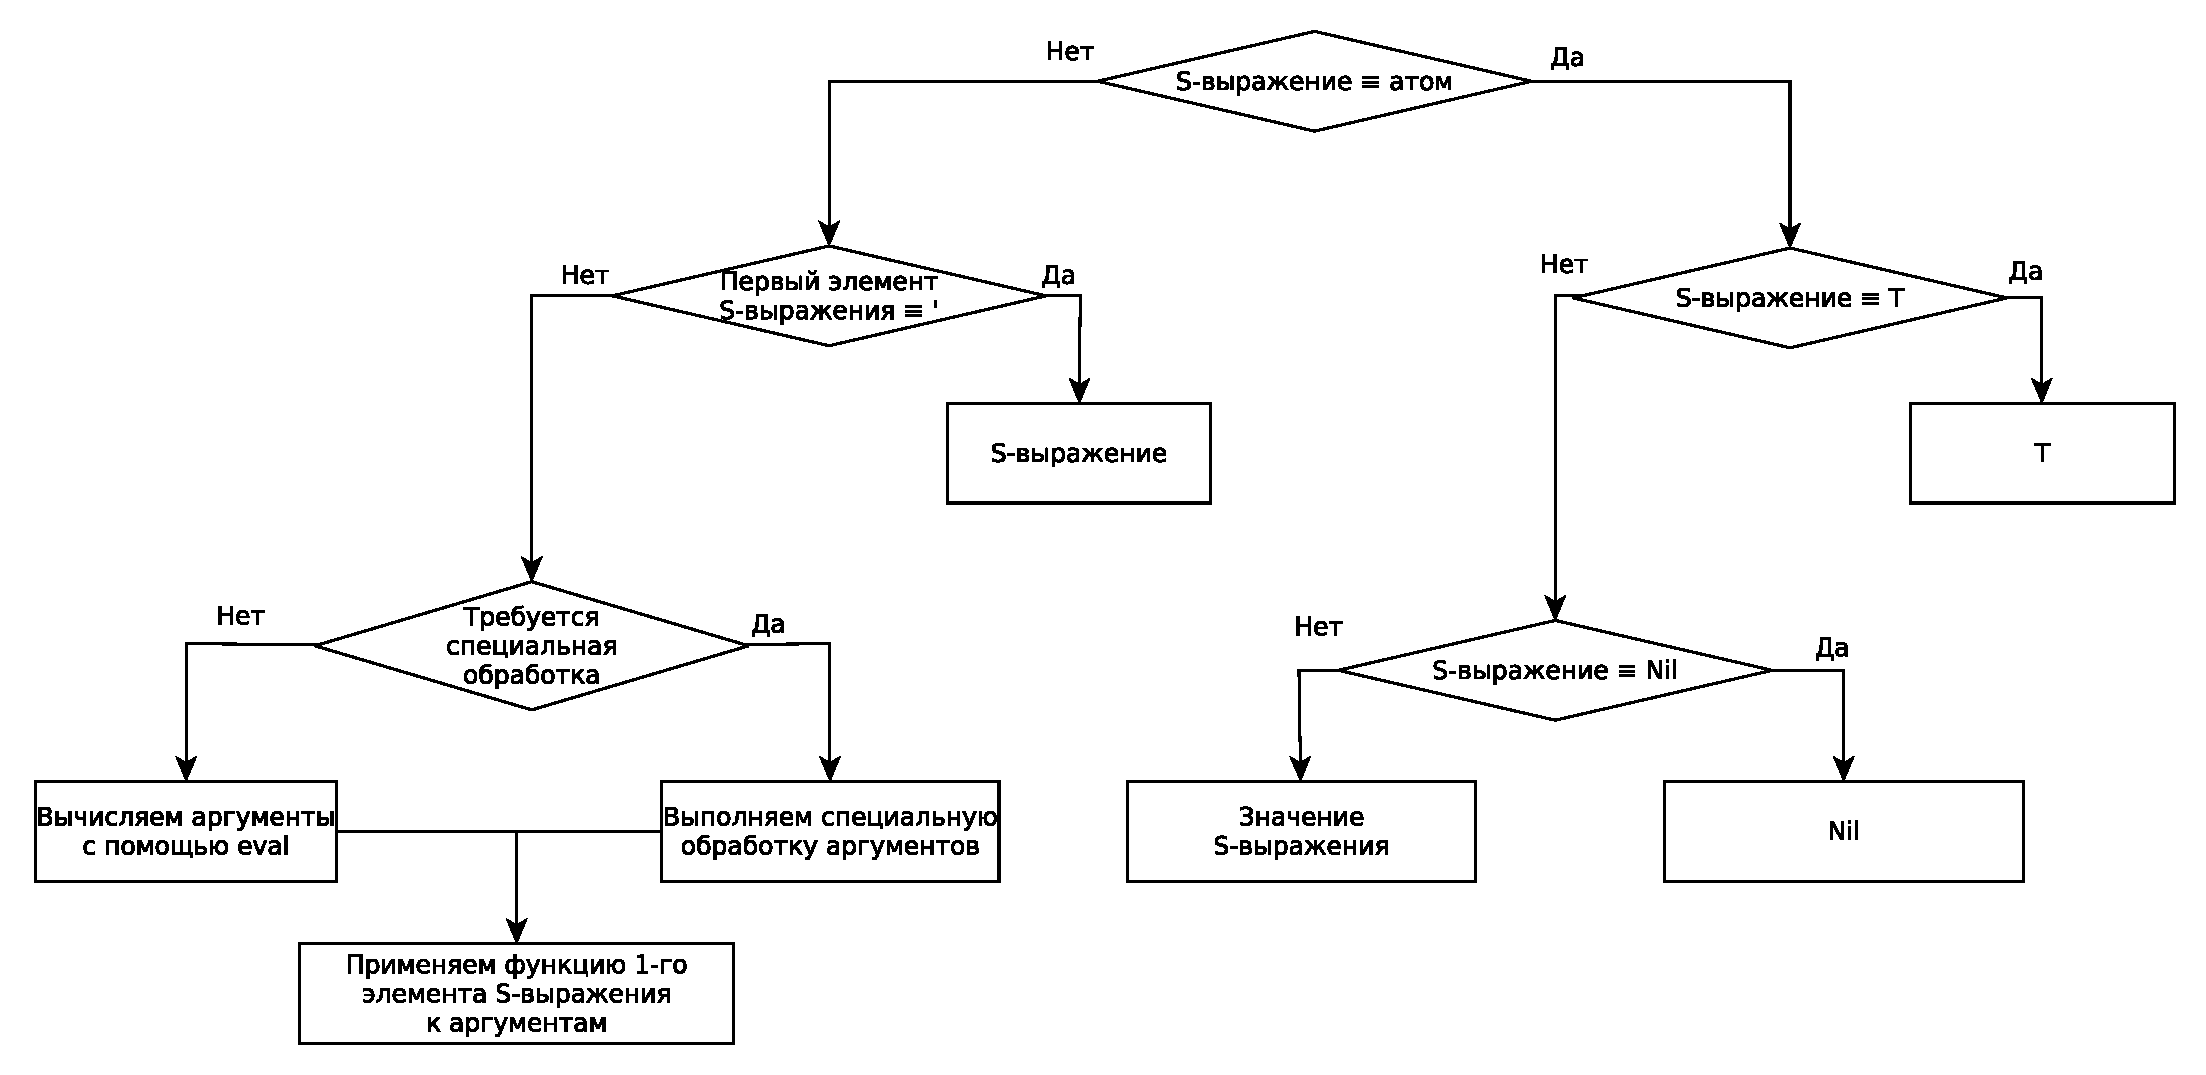
\includegraphics[width=\linewidth]{inc/img/schema}

\end{document}
